% for slides
%\documentclass[pdf,xcolor=table,envcountsect]{beamer}


% for handout
\documentclass[pdf,xcolor=table,envcountsect,handout]{beamer}


\usepackage{qtree}
\usepackage{hyperref}
\usepackage{color}
\usepackage{proof}
\usepackage{tipa}

\usepackage{graphbox}

\usepackage{tikz}
\usetikzlibrary{calc}

\newcommand{\boundellipse}[3]% center, x rad, y rad
{(#1) ellipse [x radius=#2,y radius=#3]
}

\usepackage{amsmath}

\usepackage{enumitem}

\setitemize{label=\usebeamerfont*{itemize item}%
  \usebeamercolor[fg]{itemize item}
  \usebeamertemplate{itemize item}}
  
\setenumerate[1]{%
  label=\protect\usebeamerfont{enumerate item}%
        \protect\usebeamercolor[fg]{enumerate item}%
        \insertenumlabel.}

\usetheme[numbering=none]{metropolis}

\setlength{\leftmargini}{.6cm}

\setbeamercolor{alerted text}{fg=amber,bg=}

\definecolor{airforceblue}{rgb}{0.36, 0.54, 0.66}
\definecolor{asparagus}{rgb}{0.53, 0.66, 0.42}
\definecolor{bluegray}{rgb}{0.4, 0.6, 0.8}
\definecolor{darkpowderblue}{rgb}{0.0, 0.2, 0.6}
\definecolor{darkelectricblue}{rgb}{0.33, 0.41, 0.47}
\definecolor{darkpastelblue}{rgb}{0.47, 0.62, 0.8}
\definecolor{glaucous}{rgb}{0.38, 0.51, 0.71}
\definecolor{lightslategray}{rgb}{0.47, 0.53, 0.6}
\definecolor{antiflashwhite}{rgb}{0.95, 0.95, 0.96}
\definecolor{amber}{rgb}{1.0, 0.49, 0.0}

\setbeamercolor*{palette primary}{use=structure,fg=antiflashwhite,bg=lightslategray!60}

\setbeamercolor*{block body example}{fg= amber,bg= amber}

\usepackage{natbib}

\definecolor{Light}{gray}{.81}
\definecolor{Lighter}{gray}{.92}
\definecolor{Dark}{gray}{.20}


\setlength{\bibsep}{0mm}
\setlength{\bibhang}{0.2in}
\bibpunct[:]{(}{)}{,}{a}{}{,}
\usepackage{gb4e}

%\exewidth{(\thexnumi)}

\usepackage{appendixnumberbeamer}

\usepackage{multimedia}

\def\bad{{\leavevmode\llap{*}}}
\def\marginal{{\leavevmode\llap{?}}}
\def\verymarginal{{\leavevmode\llap{??}}}
\def\infelic{{\leavevmode\llap{\#}}}


\def\centerarc<#1>[#2](#3)(#4:#5:#6)% Syntax: [overlay options] [draw options] (center) (initial angle:final angle:radius)
    { \draw<#1>[#2] ($(#3)+({#6*cos(#4)},{#6*sin(#4)})$) arc (#4:#5:#6); }


\renewcommand{\ni}{\~{\i}}
\newcommand{\yi}{\'{\symbol{16}}}
\newcommand{\nasi}{\~{\symbol{16}}}
\newcommand{\hina}{h\nasi na}
\newcommand{\ina}{\nasi na}

\newcommand{\foc}{$_{\mbox{\sc f}}$}

\usepackage{multicol,multirow,bigdelim}


\setlength{\unitlength}{1cm}

%\let\reallydohead\dohead
%\newenvironment{nonavigation}
%                   {\let\dohead\relax}
%                   {\let\dohead\reallydohead}

%\renewcommand{\bibsection}{\section*{\bibname } }
    
\setbeamercolor{title separator}{fg=amber}

\usepackage{lmodern}
\renewcommand*\familydefault{\sfdefault} % use lmodern for paragraphs
\usepackage[T1]{fontenc} % i.a. makes title font non-serif

%\setbeamertemplate{footline}[text line]{%
%  \parbox{\linewidth}{\vspace*{-8pt}Language and Information\hfill\insertshortauthor}}

\setbeamerfont{itemize/enumerate body}{size=\normalsize}
\setbeamerfont{itemize/enumerate subbody}{size=\normalsize}
\setbeamerfont{itemize/enumerate subsubbody}{size=\normalsize}

\newcommand{\specialcell}[2][c]{%
  \begin{tabular}[#1]{@{}c@{}}#2\end{tabular}}
  
%\renewcommand{\baselinestretch}{1.1}

%\setbeamersize{text margin left=0.1em} 
%\setbeamersize{text margin right=0.1em}

\title{On the information-structure sensitivity of projective content}

\author[Judith Tonhauser]{{\bf Judith Tonhauser} \\ Stuttgart University / The Ohio State University}

\date{\vspace*{1cm} Sinn und Bedeutung 23, Barcelona \\ September 5, 2018 
% \\[.5cm] \hspace*{1cm}  
%\begin{tabular}{lcr}
%  \includegraphics[width=5cm]{/Users/tonhauser.1/Pictures/stuttgart-logo}
%  \vspace{0pt} \includegraphics[width=1cm]{/Users/tonhauser.1/Pictures/osu-logo} &
%  \vspace{0pt} \includegraphics[width=1.5cm]{/Users/tonhauser.1/Pictures/nsf}
%\end{tabular}
}


%\titlegraphic{\vspace*{7cm}\includegraphics[width=1cm]{osu-logo}\hspace*{3cm}~%
%   \vspace*{.2cm}\includegraphics[width=1.4cm]{nsf}\hspace*{3cm}~%
%   \includegraphics[width=1.4cm]{acls2}
%}

\let\otp\titlepage
\renewcommand{\titlepage}{\otp\addtocounter{framenumber}{-1}}

\begin{document}

\begin{frame}[plain]

\maketitle

\end{frame}

\begin{frame}
\frametitle{Projective content}

Projective content is utterance content that listeners take speakers to be committed to even when the expression that contributes the content occurs in an entailment-canceling environment. 



\pause

\begin{exe}

\exi{(1)} Is Sam visiting Barcelona again? \hfill [{\em again} utterance]
\\ $\leadsto$ Sam has visited Barcelona before 

\pause
\bigskip

\exi{(2)} Did Sam shout WILDLY? \hfill [manner adverb utterance]
\\ $\leadsto$ Sam has been shouting

\end{exe}

\pause
\bigskip

{\bf Big question:} Why does projective content project?

\end{frame}

\begin{frame}
\frametitle{Lexicalist projection analyses for {\em again} utterances}


\hfill \begin{tiny} (e.g., \citealt{heim83,vds92,blutnerjager,beck2006,abrusan2013b})\end{tiny}
\vspace*{-.2cm}

\begin{exe}
\exi{(1)} Is Sam visiting Barcelona again?
\end{exe}

\pause

{\em again} introduces an anaphoric definedness constraint, i.e., a presupposition:

\begin{exe}
\exi{(3)} {\em again}$(p)(t)$ presupposes $p(t')$ where $t' \prec t$
\end{exe}

(1) is defined iff Sam has visited Barcelona before. If defined, (1) asks whether Sam is visiting Barcelona right now.

\medskip
\pause

Predictions of these analyses:

\begin{itemize}[topsep=-5pt,leftmargin=5ex]

\item The projectivity of the prejacent of {\em again} is at ceiling (``hard trigger'', no contextual suspension).

\item Projectivity is not sensitive to information-structural focus.

%\item Focus on {\em again} rules out restitutive interpretation:
%
%\begin{exe}
%\exi{(X)} I forgot the title of the movie AGAIN.\\[-.2cm] \hfill \begin{tiny} (adapted from \citealt[277]{beck2006}) \end{tiny}
%\end{exe}

\end{itemize}
\end{frame}

\begin{frame}
\frametitle{Empirical evidence for lexicalist projection analyses}

Paraguayan Guaran\'i (Tup\'i-Guaran\'i) 

\vspace*{-.2cm}

\begin{exe}

\exi{(4)} Context: I introduce my friend Jos\'e to you. \gll K\'ova che-angiru Jos\'e. \# O-visita {\bf jey} ch\'eve. \\ this my-friend Jose {} 3-visit again me \\ \glt `This is my friend Jose. \# He is visiting me {\bf again}.'

\pause

\exi{(5)} Context: ...who you know visited me last year. \gll K\'ova che-angiru Jos\'e. O-visita {\bf jey} ch\'eve. \\ this my-friend Jose 3-visit again me \\ \glt `This is my friend Jose. He is visiting me {\bf again}.'

\end{exe}

\medskip
This minimal pair shows that Guaran\'i {\em jey} `again' and English {\em again} are associated with an anaphoric definedness constraint. \\[-.2cm] \hfill \begin{tiny} (Strong Contextual Felicity constraint, \citealt{brst-lang11}; see also \citealt{tiemann-etal11,tiemann-etal14})\end{tiny}

\end{frame}

\begin{frame}
\frametitle{Focus-based projection analyses for manner adverb utterances}

\begin{tiny} (e.g., \citealt{simons01},Beaver 2010 [2002]\nocite{beaver-belly}, \citealt{abrusan2013,brst-ar,best-question,stevens-etal2017}) \end{tiny}

\begin{exe}
\exi{(2)} Did Sam shout WILDLY?
\end{exe}

\pause

\begin{itemize}[topsep=-5pt,leftmargin=5ex]

\item Prosody provides a cue to {\em wildly} being an information- structural focus.

\pause

\item Focus on {\em wildly} indicates (2) addresses a background question `How did Sam shout?', which entails that Sam shouted. 

\pause

\item Interlocutors are taken to be committed to this background entailment, i.e., the prejacent projects.

\end{itemize}

\bigskip
\pause

Predictions of these analyses:

\begin{itemize}[topsep=-3pt,leftmargin=5ex]

\item Projectivity is sensitive to information-structural focus.

\item The prejacent is not categorically projective. 

\end{itemize}

\end{frame}

\begin{frame}
\frametitle{Evidence for a focus-based analysis of projection}

\begin{enumerate}

\item Reported intuition that projectivity depends on information- structural focus: \begin{tiny} (see \citealt{abrusan2013} for syntactically-marked focus) \end{tiny}

\begin{exe}
\exi{(6)} Did SAM shout wildly?
\end{exe}

\medskip
\pause

\item No empirical evidence for an anaphoric definedness constraint:

\begin{exe}
\exi{(7)} Context: I couldn't see Berit during my talk. After my talk, a friend tells me: \\ Berit was smiling ironically.
\end{exe}

\medskip
\pause

\item It is implausible to lexically specify projective content in the lexical entry of all manner adverbs and other verbal modifiers.

\medskip


\end{enumerate}

\end{frame}

\begin{frame}
\frametitle{Lexicalist versus focus-based projection analyses}

\hspace*{-.5cm} \begin{tabular}{lp{5.1cm} | cc}

& & {\bf lexicalist} & {\bf focus-based} \\

& & ({\em again}) & (manner adverbs) \\ \hline

1.  & Is lexical specification plausible? & yes & no  \\[.2cm]

\pause

2. & How projective is the content? & categorical & not categorical  \\[.2cm]

\pause

3. & Is projection sensitive to information-structural focus? & no & yes  \\


\end{tabular}
\vspace*{-.2cm} \hfill \begin{tiny} (e.g., \citealt{beck2006,abrusan2013,abrusan2013b,stevens-etal2017}) \end{tiny}

\vspace*{1cm}
\pause

{\bf Empirical gap:} There is no experimental evidence comparing the projectivity or information-structure sensitivity of the projective content of {\em again} and of manner adverb utterances.


\end{frame}


\begin{frame}
\frametitle{Deciding between projection analyses}

For any given projective content, is a lexicalist or a focus-based analysis appropriate? (Or some other analysis?)

\pause

\begin{exe}
\exi{(8)} Did Sam discover that it's currently raining?
\\ $\leadsto$ it's currently raining 

\pause

\exi{(9)} Did Sam stop admiring the Sagrada Familia?
\\ $\leadsto$ Sam has been admiring the Sagrada Familia

\end{exe}

\medskip
\pause

\begin{itemize}[topsep=-1ex]

\item Lexical specification of a presupposition \hfill \begin{tiny} (e.g., \citealt{heim83,vds92}) \end{tiny}

\item Focus-based/-sensitive analyses \hfill \begin{tiny} (e.g., \citealt{abrusan2011,abrusan2016,best-question}) \end{tiny}

\item Analyses based on lexically-specified alternatives \\[-.2cm] \hfill \begin{tiny} (e.g., \citealt{abusch10,romoli2015}) \end{tiny}

\end{itemize}

\pause
\bigskip

{\bf Question:} Does the projectivity and information-structure sensitivity of these projective contents motivate a lexicalist or a focus-based analysis? (Or some other analysis?)

\end{frame}

\begin{frame}
\frametitle{This talk}


Explore and compare properties of projective content to evaluate the empirical adequacy of different projection analyses.

\pause
\vspace*{-.3cm}

\begin{exe}
\exi{(1)} Is Sam visiting Barcelona again? \hfill [lexicalist]

\exi{(2)} Did Sam shout WILDLY? \hfill [focus-based]

\exi{(8)} Did Sam discover that it's currently raining?

\exi{(9)} Did Sam stop admiring the Sagrada Familia?

\end{exe}

\medskip
\pause

Main findings: 

\vspace*{-.3cm}

\begin{enumerate}[itemsep=-1pt]

\item Lexicalist projection is influenced by utterance prosody. 

\item Focus-based projection interacts with general reasoning and conventional contributions to projection.

\end{enumerate}

\hspace*{1cm} \fbox{\begin{minipage}{8cm}{\bf Upshot:} Projection analyses need to incorporate information from multiple sources.\end{minipage}}

\end{frame}

\begin{frame}
\frametitle{Talk outline}

For any given projective content, is a lexicalist or a focus-based analysis appropriate? Or some other analysis?

\begin{itemize}

\item[1.] Is there empirical evidence for lexical specification of the projective content of utterances with {\em stop} and clause-embedding predicates like {\em discover}?

\bigskip

\item[2.] What do experimental investigations of the projectivity and information-structure sensitivity of projective content reveal? 

\bigskip

\item[3.] Discussion of the theoretical implications of the findings

\end{itemize}

\end{frame}


\begin{frame}
\frametitle{Talk outline}

For any given projective content, is a lexicalist or a focus-based analysis appropriate? Or some other analysis?

\begin{itemize}

\item[1.] \color{amber}Is there empirical evidence for lexical specification of the projective content of utterances with {\em stop} and clause-embedding predicates like {\em discover}?\color{black}

\bigskip

\item[2.] What do experimental investigations of the projectivity and information-structure sensitivity of projective content reveal? 

\bigskip

\item[3.] Discussion of the theoretical implications of the findings

\end{itemize}

\end{frame}

\begin{frame}
\frametitle{Empirical evidence for lexicalist projection analyses}

Paraguayan Guaran\'i (Tup\'i-Guaran\'i) 

\vspace*{-.2cm}

\begin{exe}

\exi{(4)} Context: I introduce my friend Jos\'e to you. \gll K\'ova che-angiru Jos\'e. \# O-visita {\bf jey} ch\'eve. \\ this my-friend Jose {} 3-visit again me \\ \glt `This is my friend Jose. \# He is visiting me {\bf again}.'


\exi{(5)} Context: ...who you know visited me last year. \gll K\'ova che-angiru Jos\'e. O-visita {\bf jey} ch\'eve. \\ this my-friend Jose 3-visit again me \\ \glt `This is my friend Jose. He is visiting me {\bf again}.'

\end{exe}

\medskip
This minimal pair shows that Guaran\'i {\em jey} `again' and English {\em again} are associated with an anaphoric definedness constraint. \\[-.2cm] \hfill \begin{tiny} (Strong Contextual Felicity constraint, \citealt{brst-lang11}; see also \citealt{tiemann-etal11,tiemann-etal14})\end{tiny}

\end{frame}

\begin{frame}
\frametitle{No empirical evidence for an anaphoric definedness constraint}

\vspace*{-.3cm}

\hfill \begin{tiny} (examples adapted from \citealt[80]{brst-lang11}, see also \citealt{spenader02,spenader03}) \end{tiny}

\vspace*{-.2cm}
\pause

\begin{exe}

\exi{(10)} Context: Laura, who doesn't live with her parents, visits them and asks them to sit down with her because she has to tell them something: 
\gll Nd-a-je-droga-v\'e-i-ma. \\ {\sc neg-}I-{\sc refl}-drug-more{\sc -neg-perf} \\ \glt `I've {\bf stopped} doing drugs.' 

\pause

\exi{(11)} Context: A girl backs out of a driveway and hits Susi's car. A woman comes running out of the house, apologizes that her daughter hit Sus's car and says: \gll Ha'e {\bf oi-kuaa} o-mo\~{\i}-va'er\~a=ha i-l\'ente o-maneja=ha-gu\~a. \\ she 3-know 3-put-must=that her-glasses 3-drive=that{\sc -purp} \\ \glt `She {\bf knows} that she has to use her glasses to drive.' 


\end{exe}
\end{frame}

\begin{frame}
\frametitle{Lexical specification doesn't predict non-detachability}

The projective content associated with `stop' and clause- embedding predicates is non-detachable, intra- and cross- linguistically. \begin{tiny}(e.g., \citealt{levinson-annamalai92,simons01,brst-lang11,tonhauser-guarani-variability}) \end{tiny}

\pause

\begin{exe}

\exi{(12)} Did Jane stop / quit / cease laughing? \\[-.2cm] \hfill \begin{tiny} (adapted from \citealt[435]{simons01}) \end{tiny}

\medskip
\pause

\exi{(13)} \gll J\'ane=pa nd-o-puka-v\'e-i-ma? \\ Jane{\sc =q} {\sc neg-}3-laugh-more{\sc -neg-perf} \\ \glt `Did Jane stop laughing?'

\medskip
\pause

\exi{(14)} \gll S\'am=pa {\bf o-topa} / {\bf oi-kuaa} o-ky=ha? \\ Sam{\sc =q} 3-discover {} 3-know 3-rain=that \\ \glt `Did Sam {\bf discover} / Does Sam {\bf know} that it's raining?'

\end{exe}

\end{frame}


\begin{frame}
\frametitle{Talk outline}

For any given projective content, is a lexicalist or a focus-based analysis appropriate? Or some other analysis?

\begin{itemize}

\item[1.] Is there empirical evidence for lexical specification of the projective content of utterances with {\em stop} and clause-embedding predicates?

\begin{itemize}[leftmargin=8ex]

\item[{\bf yes}] {\em again} (lexicalist analysis)

\item[{\bf no}] manner adverbs (focus-based analysis) 
\pause
\\ {\em stop} \\ clause-embedding predicates

\end{itemize}

\bigskip
\pause

\item[2.] \color{amber}What do experimental investigations of the projectivity and information-structure sensitivity of projective content reveal?\color{black}

\bigskip

\item[3.] Discussion of the theoretical implications of the findings

\end{itemize}

\end{frame}

%\begin{frame}
%\frametitle{Findings of previous experimental investigations}
%
%\begin{itemize}[leftmargin=1ex]
%
%\item \citealt{xue-onea11}: The prejacent of German {\em wieder} `again' is categorically projective.
%
%\medskip
%
%\item \citealt*{stevens-etal2017}: The prejacent of English manner adverb utterances is weakly projective and projectivity is sensitive to prosodically-marked focus.
%
%\medskip
%
%\item \citealt*{tbd-variability}: The projective content of {\em stop} and of some clause-embedding predicates is less than categorically projective.
%
%\medskip
%
%\item \citealt{tonhauser-salt26}: The projectivity of the content of the complement of English clause-embedding predicates is sensitive to prosodically-marked focus.
%
%\end{itemize}
%
%
%\end{frame}

%\begin{frame}
%\frametitle{Projective content doesn't have to project}
%
%Judgments on naturally occurring data from CommitmentBank: \\[-.2cm]  \hfill \begin{tiny} (\citealt{demarneffe-etal2018}) \end{tiny}
%
%\medskip
%
%\begin{exe}
%
%\exi{(X)} At the heart of the universe there is cruelty. We are predators and preyed upon, every living thing. Did you know that wasps lay their eggs in ladybirds? \hfill [3]
%
%\medskip
%
%\exi{(X)} Willy did mention it.\ I was puzzled, I'll admit, but now I un- derstand.\ How did you know Heather had been there? [1.4]
%
%\medskip
%
%\exi{(X)} Rather a long shot wasn't it? Twenty years? How do you know the baby was born here? \hfill [0]
%
%\end{exe}
%
%\bigskip
%
%Projectivity is a gradient property of utterance content.\\[-.2cm] \hfill \begin{tiny} (\citealt{tbd-variability,tonhauser-degen,demarneffe-etal2018}) \end{tiny}
%
%\end{frame}
%
%\begin{frame}
%\frametitle{Projectivity is a gradient property of utterance content}
%
%{\bf CommitmentBank:} 122 discourses with {\em know}
%
%$\approx$ 9 ratings per discourse
%
%\medskip
%\pause
%
%\includegraphics[width=.85\paperwidth]{/Users/tonhauser.1/Documents/current-research-topics/database/analysis/graphs/item-means-of-know}
%
%There is both by-item and by-participant variability.
%
%\end{frame}

\begin{frame}
\frametitle{German {\em wieder} `again' (\citealt{xue-onea11})}

\pause

\begin{exe}
\exi{(15)} Wenn Thomas wieder Sushi macht, hilft Maiko dabei.
\\ `If Thomas again makes sushi, Maiko will help him.'
\end{exe}

{\bf Question to participants:} \\[-.1cm] \hspace*{1cm} Is it possible that Thomas hasn't made sushi before?

\bigskip
\pause

{\bf Findings:} \hspace*{1cm} \begin{tabular}[t]{lr}
	& \% `no' responses \\\hline
	\pause
{\em wieder} `again' & 99\%  \\
\pause
{\em auch} `too' & 87\% \\ 
{\em erfahren} `find out' & 52\% \\
{\em wissen} `know' & 38\%
\end{tabular}

\bigskip

The projective content associated with {\em wieder} `again' is highly projective, as expected from lexicalist projection analyses.

\end{frame}


%\begin{frame}
%
%\frametitle{English manner adverb utterances \\[-.1cm] \hfill (\citealt*{stevens-etal2017})}
%
%\begin{exe}
%\exi{(X)} Sally: Amanda didn't clap loudly.
%\end{exe}
%
%{\bf Question to participants:} \\[-.1cm] \hspace*{1cm} Is Sally certain that Amanda has clapped? 
%
%\medskip
%
%\begin{tabular}{lll}
%{\bf Findings:} & \hspace*{.5cm} & \includegraphics[align=t,width=.42\paperwidth]{/Users/tonhauser.1/Documents/current-research-topics/NSF-NAI/prop-att-experiments/6-prosody-manner-advs/results/graphs/mean-projectivity-by-control-and-target} \\
%\end{tabular}
%
%\medskip
%
%The projective content associated with manner adverb utterances is only weakly projective, in line with a focus-based analysis.
%
%\end{frame}

\begin{frame}
\frametitle{English manner adverb utterances \\[-.1cm] \hfill \begin{small} (\citealt*{stevens-etal2017})\end{small}}

\vspace*{-.2cm}
\begin{exe}
\exi{(16)} Sally: Amanda didn't clap loudly.
\pause
\\ 1. \hspace*{.7cm} \color{amber}L+H*\color{black} \hspace*{3.1cm} L-L\% \hspace*{.3cm} [name focus]
\pause
\\ 2. \hspace*{3.8cm} \color{amber}L+H*\color{black}{} L-L\% \hspace*{.3cm} [adverb focus]
\end{exe}

\pause

{\bf Question to participants:} \\[-.1cm] \hspace*{1cm} Is Sally certain that Amanda has clapped? 

\medskip
\pause

\hspace*{-.3cm} \begin{tabular}{lll}
{\bf Findings:} & \hspace*{.2cm} & \includegraphics[align=t,width=.4\paperwidth]{/Users/tonhauser.1/Documents/current-research-topics/NSF-NAI/prop-att-experiments/6-prosody-manner-advs/results/graphs/mean-projectivity-by-control-and-prosody} \\
\end{tabular}

\medskip

Projectivity is not categorical and sensitive to focus.

\end{frame}


\begin{frame}
\frametitle{English {\em stop} and clause-embedding predicates \\[-.1cm] \hfill \begin{small}(\citealt*{tbd-variability})\end{small}}

\begin{small}
\begin{exe}
\exi{(17)} Sally: Did Mary's daughter {\bf stop} biting her nails?

\exi{(18)} Sally: Did Sam {\bf discover} / Does Sam {\bf know} / Is Sam {\bf annoyed}
\\ \hspace*{1cm} ...that Mary's daughter has been biting her nails?

\end{exe}
\end{small}

\pause

\vspace*{-.2cm}

{\bf Question to participants:} \\[-.1cm]  \begin{small} Is Sally certain that Mary's daughter has been biting her nails? \end{small}

\medskip
\pause

\hspace*{-.3cm} \begin{tabular}{lll}
{\bf Findings:} & \hspace*{.5cm} & \includegraphics[align=t,width=.5\paperwidth]{/Users/tonhauser.1/Documents/current-research-topics/NSF-NAI/prop-att-experiments/1factive-verbs/Git-variability/results/exp1a/graphs/mean-projectivity-by-control-and-stop-and-factives} \\
\end{tabular}

The content associated with {\em stop} and {\em discover} is less projective than that of {\em know} and {\em be annoyed}.

\end{frame}

\begin{frame}
\frametitle{English clause-embedding predicates  \hfill \begin{small}(\citealt{tonhauser-salt26})\end{small}}

\vspace*{-.2cm}
\begin{exe}
\exi{(19)} Perhaps she knew that he was wrong.
\pause
\\ 1. \hspace*{1.8cm} \color{amber}H*\color{black} \hspace*{3.15cm} L-L\%   \hfill \begin{small} [predicate foc]\end{small}
\pause
\\ 2. \hspace*{4.4cm} \color{amber}L+H*\color{black} \hspace*{.05cm} L-L\% \hfill \begin{footnotesize} [complement foc]\end{footnotesize}

\end{exe}

\pause

{\bf Question to participants:} \hfill Is Sally certain that he was wrong? 

\medskip
\pause

\hspace*{-.3cm} \begin{tabular}{lll}
{\bf Finding:} & \hspace*{.5cm} & \includegraphics[align=t,width=.5\paperwidth]{/Users/tonhauser.1/Documents/current-research-topics/NSF-NAI/prop-att-experiments/5-prosody-factives/3-perception-1a/results/graphs/mean-projectivity-by-prosody} \\
\end{tabular}

Projectivity is sensitive to prosodically-marked focus.\\[-.2cm] \hfill \begin{tiny} (see also \citealt{djaerv-bacovcin-salt27}) \end{tiny}

\end{frame}

\begin{frame}
\frametitle{Summary of available empirical evidence}

\begin{itemize}
\item[2.] What do experimental investigations of the projectivity and information-structure sensitivity of projective content reveal?
\end{itemize}

\bigskip

\begin{tabular}{l l | c c} 

& & {\bf Categorical} & {\bf Focus-} \\[-.1cm] 
analysis & & {\bf projectivity?} & {\bf sensitivity?} \\\hline\hline

lexicalist & {\em wieder} `again' & yes & \color{amber}?\color{black} \\

& {\em again} & \color{amber}?\color{black} & \color{amber}?\color{black} \\

\hline
\pause


focus & manner adverbs & no & yes \\

\hline
\pause

& clause-emb preds & yes/no & yes \\

& {\em stop} & no & \color{amber}?\color{black} \\


\hline
\end{tabular}

\pause

\vspace*{.5cm}

Further short-comings of the available empirical evidence:

\begin{itemize}[topsep=-10pt,leftmargin=5ex]

\item No cross-content comparison

\item Different response tasks 

\end{itemize}

\end{frame}


\begin{frame}
\frametitle{Comprehension experiment}

With Marie-Catherine de Marneffe, Shari R.\ Speer and Jon Stevens

\medskip
\pause

{\bf Research questions:} How projective are different contents? Is their projectivity sensitive to prosodically-marked focus?

\medskip

\begin{exe}
\exi{(20)}

\begin{xlist}

\ex Did Alfie text again? \hfill [lexicalist] \\ $\leadsto$ Alfie texted before

\ex Did Alfie text secretly? \hfill [focus-based] \\ $\leadsto$ Alfie texted

\ex Did Alfie stop texting? \\ $\leadsto$ Alfie texted before
 
\end{xlist}

\end{exe}

\medskip

\pause

176 participants recruited on Amazon's Mechanical Turk platform

\end{frame}

\begin{frame}
\frametitle{Same projective content across the three types of expressions}

\pause

\begin{exe}
\exi{(21)}

\begin{xlist}

\ex Did Alfie text again when Dan arrived? \\ $\leadsto$ Alfie texted before Dan arrived

\pause


\ex Did Alfie stop texting when Dan arrived? \\ $\leadsto$ Alfie texted before Dan arrived

\pause

\ex Did Alfie text secretly before Dan arrived? \\ $\leadsto$ Alfie texted before Dan arrived

\end{xlist}

\end{exe}

\pause

{\bf Question to participants:} \\[-.1cm] \hspace*{.5cm} Is Sally certain that Alfie texted before Dan arrived? 

\medskip
\pause

\underline{Target sentences:}
\\
36 triples like (21), 3 for each of the 12 verbs ({\em text, smile, walk,...})
\\
108 sentences total

\end{frame}

\begin{frame}
\frametitle{Spoken stimuli with prosodically-marked focus}

4 prosodic conditions: L* pitch accent, H-H\% boundary tone

\pause

\begin{itemize}[leftmargin=2ex]
\item[] {\bf Aux:}  DID Alfie text again when Dan arrived? \hfill \movie[inlinesound,samplingrate=8000,encoding=Raw,bitspersample=16,channels=1]
{\beamerbutton{Play Sound}}{sounds/alfie-text-a-A.aiff} 

\item[] {\bf Subject:} Did ALFIE text again when Dan arrived? \hfill \movie[inlinesound,samplingrate=8000,encoding=Raw,bitspersample=16,channels=1]
{\beamerbutton{Play Sound}}{sounds/alfie-text-a-S.aiff}

\item[] {\bf Verb:} Did Alfie TEXT again when Dan arrived? \hfill \movie[inlinesound,samplingrate=8000,encoding=Raw,bitspersample=16,channels=1]
{\beamerbutton{Play Sound}}{sounds/alfie-text-a-V.aiff}

\item[] {\bf Target:} Did Alfie text AGAIN when Dan arrived? \hfill \movie[inlinesound,samplingrate=8000,encoding=Raw,bitspersample=16,channels=1]
{\beamerbutton{Play Sound}}{sounds/alfie-text-a-T.aiff}

\end{itemize}

\medskip
\pause

108 sentences x 4 prosodic conditions = 432 utterances

\medskip
\pause

Prosodic variation was reduced by using the same temporal adjunct clause recording in each set of 4

\medskip
\pause

36 utterances per participant: 12 for each content type ({\em again, stop}, manner), 3 per prosodic condition (within-participant factors)

\end{frame}

\begin{frame}
\frametitle{Procedure}

Imagine that you are at a party. Upon walking into the kitchen, you overhear Debby, the party host, ask another guest a question.

\movie[inlinesound,samplingrate=8000,encoding=Raw,bitspersample=16,channels=1]
{\beamerbutton{Play Sound}}{sounds/annie-clean-m-S.aiff} 

\vspace*{1cm}

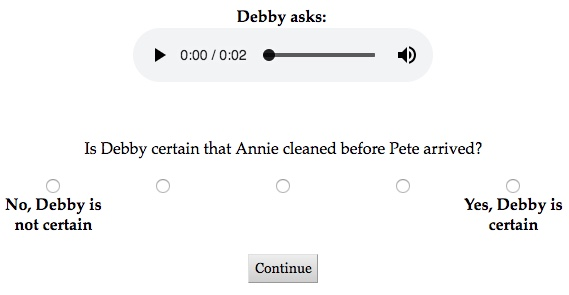
\includegraphics[width=10cm]{/Users/tonhauser.1/Documents/current-research-topics/NSF-NAI/prop-att-experiments/8-stop-again-manner/paper/pictures/trial}  

\end{frame}

\begin{frame}
\frametitle{Statistical analyses}

Ordinal mixed effects models 

\begin{itemize}[topsep=-1ex,leftmargin=5ex,itemsep=-1pt]

\item Predict certainty rating from content type / prosodic condition 

\item Random effects: participant, item, content

\item Slope: participant
 
\end{itemize}

\bigskip
\pause

Results based on data from 126 participants \begin{small} (ages 21-76; mean: 36)\end{small}

Data exclusion:

\begin{itemize}[topsep=-1ex,leftmargin=5ex,itemsep=-1pt]

\item 5 self-declared non-native speakers of American English %(176-5 = 171)

\item 6 participants who always responded `1' %(171 - 6 = 165)

\item 39 participants with response mean $>$ 2 for the four main clause control stimuli \begin{footnotesize}(no change in findings if these data included)\end{footnotesize}

\end{itemize}

\end{frame}

\begin{frame}
\frametitle{Research questions}

\begin{enumerate}

\item How projective are the projective contents?

\medskip

\item Is projectivity sensitive to prosodically-marked information-structural focus?

\end{enumerate}

\end{frame}

\begin{frame}
\frametitle{How projective are the projective contents?}

\hfill \begin{footnotesize} [1512 data points / target content, collapsing over the 4 prosodic conditions] \end{footnotesize}

\pause

\hspace*{1cm} 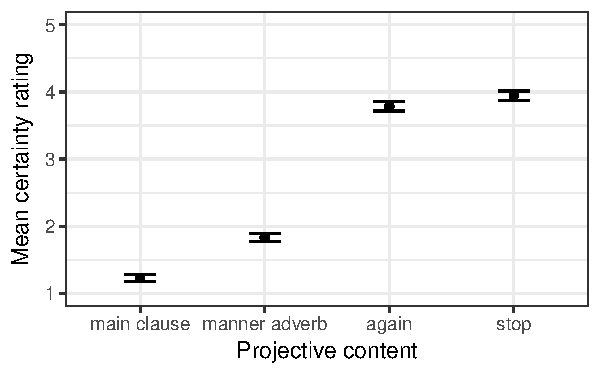
\includegraphics[width=8cm]{/Users/tonhauser.1/Documents/current-research-topics/NSF-NAI/prop-att-experiments/8-stop-again-manner/results/graphs/means-projectivity-by-expression}

\pause

{\bf $\checkmark$} Prejacent of manner adverb utterances is weakly projective.
\\[.02cm]
{\bf $\checkmark$} Prejacent of {\em again} utterances is much more projective.
\\[.02cm]
\pause
{\bf $\times$} The projectivity of none of the contents is at ceiling.
\\[.02cm]
{\bf $\times$} Pre-state of {\em stop} is more projective than prejacent of {\em again}.


\end{frame}

\begin{frame}
\frametitle{Is projectivity sensitive to prosodically-marked focus?}

Predictions of the focus-based projection analysis for the prejacent of manner adverb utterances: \hfill \begin{tiny} (e.g., \citealt{abrusan2013,best-question,stevens-etal2017}) \end{tiny}

\pause

\begin{enumerate}

\item Prejacent is projective but not categorically so when the manner adverb is in focus

{\bf Target:} Did Alfie text SECRETLY?
\pause
\\ Background question: \{Alfie texted x $|$ x is a verb modifier \}
\pause
\\ entails: Alfie texted

\pause

\item Prejacent is not projective when another expression is in focus

{\bf Subject:} Did ALFIE text secretly?
\pause
\\ Background question: \{x texted secretly $|$ x an individual\}
\pause
\\ doesn't entail that Alfie texted

\medskip
\pause

{\bf Aux:}  DID Alfie text secretly?
\\
{\bf Verb:} Did Alfie TEXT secretly?

\end{enumerate}

\end{frame}

\begin{frame}
\frametitle{Results: Prejacent of manner adverb utterances}

\hfill \begin{footnotesize} [378 data points per prosodic condition] \end{footnotesize}
\hspace*{1cm} 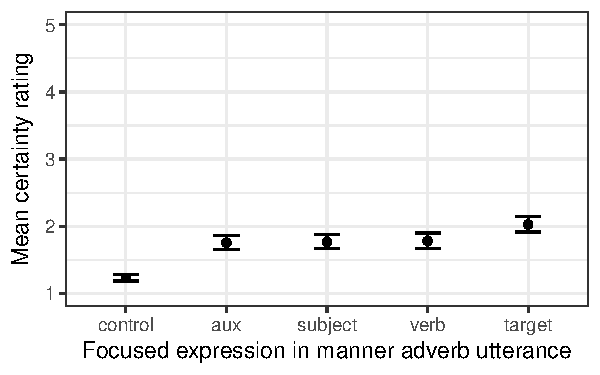
\includegraphics[width=8cm]{/Users/tonhauser.1/Documents/current-research-topics/NSF-NAI/prop-att-experiments/8-stop-again-manner/results/graphs/mean-projectivity-manner-by-prosody}


\vspace*{.6cm}
\pause

{\bf $\checkmark$} Prejacent is more projective with focus on the manner adverb. 
\\[.1cm]
\pause
{\bf $\times$} Prejacent is weakly projective in all prosodic conditions. \\[-.2cm] \hfill \begin{tiny} (see also \citealt{stevens-etal2017}) \end{tiny}




\end{frame}

\begin{frame}
\frametitle{Is projectivity sensitive to prosodically-marked focus?}

Prediction of the lexicalist projection analysis for the prejacent of {\em again} utterances: \hfill \begin{tiny} (e.g., \citealt{beck2006,abrusan2013b}) \end{tiny}


Projectivity of prejacent is at ceiling regardless of which expression is in focus.

\end{frame}

\begin{frame}
\frametitle{Results: Prejacent of {\em again} utterances}

\hfill \begin{footnotesize} [378 data points per prosodic condition] \end{footnotesize}
\hspace*{1cm} 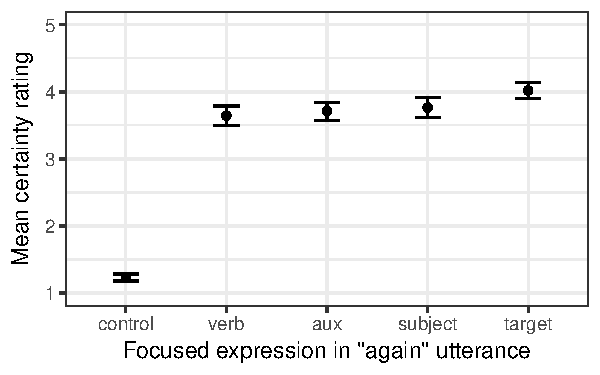
\includegraphics[width=8cm]{/Users/tonhauser.1/Documents/current-research-topics/NSF-NAI/prop-att-experiments/8-stop-again-manner/results/graphs/mean-projectivity-again-by-prosody}

\bigskip
\pause

{\bf $\times$} Projectivity of prejacent of {\em again} utterances is not at ceiling.
\\[.1cm]
{\bf $\times$} Prejacent is more projective with focus on {\em again}.

\end{frame}

\begin{frame}
\frametitle{Focus-sensitivity for pre-state of {\em stop} utterances}

\begin{itemize}[topsep=-2pt,leftmargin=2ex]

\item {\bf Default projection} (\citealt{abusch10,abrusan2011,abrusan2016,romoli2015}): pre-state projects by default (lexically specified alternatives, backgrounded entailment, obligatory scalar implicature), unless contextually defeated. 
\pause
\\ Predictions:
\begin{itemize}
\item[--] Focus on {\em stop}: projectivity of pre-state at ceiling
\item[--] Focus elsewhere: pre-state less projective
\end{itemize}

\pause

\item {\bf Focus-based projection} \begin{small}(e.g., \citealt{best-question,brst-ar}):\end{small}
\\ Same predictions as for manner adverb utterances:
\pause
\begin{itemize}
\item[--] Pre-state is projective but not categorically so with focus on {\em stop}
\item[--] Pre-state is not projective with focus on another expression
\end{itemize}

\end{itemize}

\end{frame}

\begin{frame}
\frametitle{Results: Pre-state content of {\em stop}}


\hfill \begin{footnotesize} [378 data points per prosodic condition] \end{footnotesize}
\hspace*{1cm} 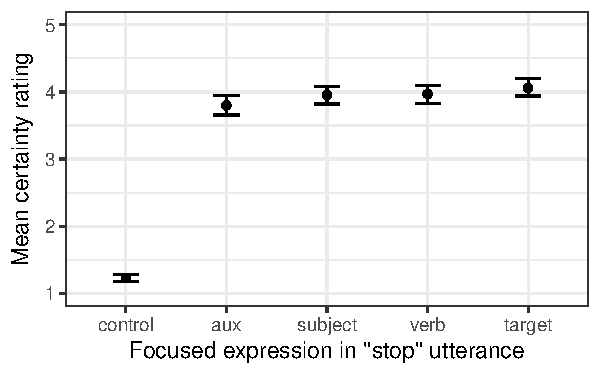
\includegraphics[width=8cm]{/Users/tonhauser.1/Documents/current-research-topics/NSF-NAI/prop-att-experiments/8-stop-again-manner/results/graphs/mean-projectivity-stop-by-prosody}

\medskip
\pause

$\bullet$ Projectivity of pre-state is high but not at ceiling. \begin{footnotesize}(neither theory)\end{footnotesize}
\\[.1cm]
\pause
$\bullet$ Pre-state content is more projective...
\\ \hspace*{.7cm} ...with focus on {\em stop} than on subject or auxiliary  \begin{footnotesize} (both) \end{footnotesize}
\pause
\\ \hspace*{.7cm} ...with focus on verb than on auxiliary \begin{footnotesize} (neither) \end{footnotesize}

\end{frame}

\begin{frame}
\frametitle{Summary of findings}

{\bf Research questions:} How projective are the contents and is their projectivity sensitive to prosodically-marked focus?

\pause
Projectivity:

\begin{itemize}[leftmargin=2ex,topsep=-1ex]

\item The projective content of manner adverb utterances is weakly projective, and that of {\em again} and {\em stop} utterance highly projective.

\item The projectivity of the content of manner adverb utterances is never at floor, and that of {\em again} utterances is never at ceiling. 

\end{itemize}

\pause

\medskip
Sensitivity to prosodically-marked focus:

\begin{itemize}[leftmargin=2ex,topsep=-1ex]

\item The projectivity of all three types of projective content is sensitive to the prosodic manipulation.

\item The sensitivity of {\em stop} utterances to the prosodic manipulation is more varied than for utterances with manner adverbs or {\em again}.


\end{itemize}


\end{frame}

\begin{frame}
\frametitle{Discussion: Which projection analyses are appropriate?}

\pause

{\bf General theme:} 

\begin{itemize}

\item Neither lexicalist nor focus-based analyses alone account for the findings.

\item Empirically adequate projection analyses need to incorporate cues from multiple sources, including:

\begin{itemize}

\item anaphoric definedness constraints

\item information structure

\item truth-conditional content

\item general reasoning and world knowledge

\item other information communicated by prosody

\end{itemize}

\begin{tiny} (see also \citealt*{tbd-variability}) \end{tiny}

\end{itemize}

\end{frame}

\begin{frame}
\frametitle{Discussion: Which projection analyses are appropriate?}


Prejacent of manner adverb utterances: weakly projective even when manner adverb is not in focus.

\pause

\begin{itemize}

\item Focus-based analysis alone does not predict this finding. 

\pause

\medskip

\item {\bf Possible way forward:} General reasoning contributes to projectivity, i.e., what we take the speaker to be committed to.

\vspace*{.6cm}
\pause

\underline{For example:}

\begin{exe}
\exi{(22)} Berit wasn't smiling.

\exi{(23)} Berit wasn't smiling ironically.
\end{exe}

By uttering (23) rather than the simpler (22), the speaker is taken to be committed to Berit having smiled.

Focus on the manner adverb strengthens commitment.



\end{itemize}

\end{frame}

\begin{frame}
\frametitle{Discussion: Which projection analyses are appropriate?}

Prejacent of {\em again} utterances: projectivity was not at ceiling (mean: 3.79 / 5) and sensitive to prosodic condition.

\pause

Projectivity not being at ceiling contrasts with finding for {\em wieder} `again' in \citealt{xue-onea11}

\pause

\begin{itemize}[topsep=-3pt]

\item 12 {\em again} items vs.\ 3 {\em wieder} `again' items

\item 126 participants vs.\ 34 participants

\item Certainty judgment vs.\ possibility of prejacent being false

\pause

\item 5-point Likert scale vs.\ binary response

\pause

\hspace*{.5cm} 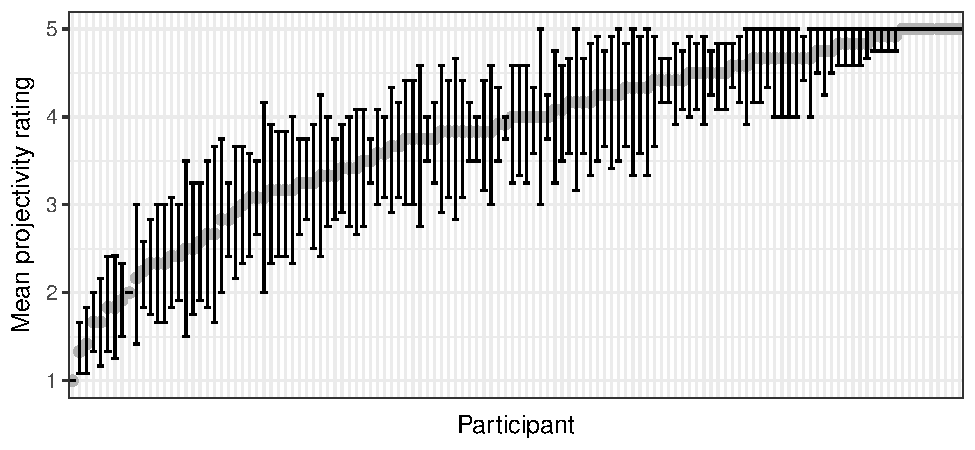
\includegraphics[width=7.8cm]{/Users/tonhauser.1/Documents/current-research-topics/NSF-NAI/prop-att-experiments/8-stop-again-manner/results/graphs/mean-projectivity-again-by-participant}

\end{itemize}

\end{frame}

\begin{frame}
\frametitle{Discussion: Which projection analyses are appropriate?}


\begin{itemize}[topsep=-5pt]

\item No currently available analysis of {\em again} allows for the suspension of the prejacent of {\em again} utterances under any circumstances (``hard trigger'').

\medskip

\item Given  evidence for anaphoric definedness constraint, we don't want to give up on anaphoric analysis. \hfill \begin{tiny}(\citealt{tiemann-etal11,tiemann-etal14} on {\em wieder})\end{tiny}

\medskip
\pause

\item {\bf Avenue for future research:} 

\begin{itemize}[leftmargin=3ex]

\item Prosody is a cue to focus but also conveys information about the speaker's epistemic and emotional state, authority, stance towards the interlocutor, politeness, etc. 

\item It is possible that this information interacts with how committed the speaker is taken to be, i.e., with the projectivity of the prejacent.  

\end{itemize}

\end{itemize}

\end{frame}

\begin{frame}
\frametitle{Discussion: Which projection analyses are appropriate?}

Pre-state of {\em stop} utterances: 

\begin{itemize}[topsep=-5pt]

\item Projectivity was not at ceiling, but higher than with manner adverb utterances.

\item Projectivity was sensitive to prosodic condition in a more fine-grained fashion than expected on focus-based analyses.

\end{itemize}

\bigskip

\pause
Should the mean rating for {\em stop} utterances be considered the ceiling? (4.1 out of 5)

No: projectivity consisted with findings of \citealt{tbd-variability}.

\hspace*{2cm} \begin{tabular}{lr}

expression & mean rating \\ \hline

{\em stop} & .87 \\

{\em know} & .92 \\

{\em NRRC} & .95 \\

{\em be annoyed} & .96 \\

\end{tabular}

\end{frame}

\begin{frame}
\frametitle{Discussion: Which projection analyses are appropriate?}

Lexicalist or default projection analyses not empirically adequate:

\begin{itemize}[topsep=-2ex,itemsep=-2pt]

\item No empirical evidence for an anaphoric definedness constraint.

\item Projectivity was not at ceiling. 
\end{itemize}

\bigskip
\pause

Focus-based analysis alone is not empirically adequate either:

\hspace*{.5cm} 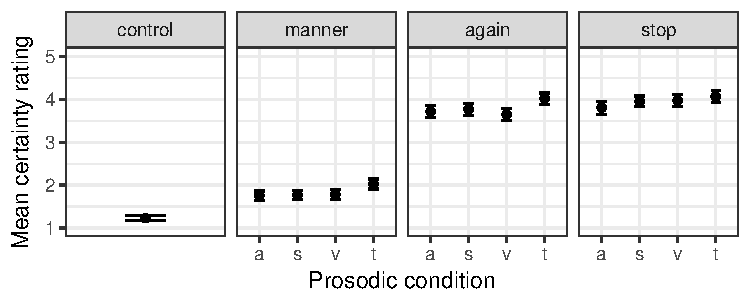
\includegraphics[width=9cm]{/Users/tonhauser.1/Documents/current-research-topics/NSF-NAI/prop-att-experiments/8-stop-again-manner/results/graphs/means-projectivity-by-expression-and-prosody}

\pause

{\bf Proposal:} Incorporate contribution from truth-conditional content of {\em stop} to projectivity. \begin{tiny} (see also \citealt{tbd-variability}) \end{tiny}

\end{frame}

\begin{frame}
\frametitle{Summary of theoretical implications}

{\bf Research questions:} Why does projective content project? For any given projective content, is a lexicalist or a focus-based analysis appropriate? (Or some other analysis?)

\pause

\begin{itemize}

\item Lexicalist and focus-based analyses do not adequately capture properties of projective contents they were designed for: {\em again} and manner adverb utterances, respectively.

\medskip
\pause

\item Likewise, the properties of the pre-state of {\em stop} utterances are not captured by any of the analyses currently on the market (lexicalist, focus-based, default-based).

\end{itemize}

\hspace*{1cm} \fbox{\begin{minipage}{8cm}{\bf Upshot:} Projection analyses need to incorporate information from multiple sources.\end{minipage}}

\end{frame}

\begin{frame}
\frametitle{Concluding remarks}


Projective content is heterogeneous and different analyses have been proposed for subclasses.

\medskip

Research over the past 50 years has revealed many factors that influence projectivity:

\begin{itemize}[topsep=-2ex,itemsep=-1pt]

\item anaphoric definedness constraints \hfill \begin{tiny} (e.g., \citealt{heim83,vds92}) \end{tiny}

\item information structure \hfill \begin{tiny} (e.g., \citealt{beaver-belly,tbd-variability}) \end{tiny}

\item truth-conditional content  \hfill \begin{tiny} (e.g., \citealt{karttunen71b,tbd-variability}) \end{tiny}

\item world knowledge  \hfill \begin{tiny} (e.g., \citealt{tonhauser-etal-eval,degen-tonhauser-prior}) \end{tiny}


\item trustworthiness of attitude holder \hfill \begin{tiny} (e.g., \citealt{schlenker10,spector-egre2015}) \end{tiny}

\item information communicated by prosody

\end{itemize}

\bigskip
\pause

Avenues for future research:

\begin{itemize}[topsep=-2ex,itemsep=-1pt]

\item Develop and test analyses that incorporate information from multiple sources.

\item Broaden empirical scope to less well-studied languages.

\end{itemize}


\end{frame}


\begin{frame}
\frametitle{Acknowledgments}

My collaborators and I thank the following agencies for the funding that supported the research presented here:

\begin{itemize}

\item National Science Foundation

\item American Council of Learned Socities

\item Ohio State University Arts \& Sciences Discovery Theme

\item Ohio State University Targeted Investment in Excellence

\end{itemize}

\end{frame}

\begin{tiny}

\bibliographystyle{/Users/tonhauser.1/Library/Latex/cslipubs-natbib}
\bibliography{/Users/tonhauser.1/Documents/bibliography}

\end{tiny}

\end{document}


